\documentclass{article}
\usepackage[utf8]{inputenc}
\usepackage{graphicx}
\usepackage{subcaption}
\usepackage{amsmath}
\usepackage[
  backend=biber,
  style=apa,
  citestyle=apa
]{biblatex}

\addbibresource{references.bib}

\title{Bayesian Networks with Applications to Simulated Macroeconomic Timeseries}
\author{Emmet Hall-Hoffarth}
\date{May 2020}

\begin{document}

\maketitle

\section{Introduction}
Bayesian networks \parencite{pearl2018book} \parencite{pearl2014probabilistic} are a non-parametric statistical technique for modelling causal probabilistic relationships. Under some conditions this and associated tools can allow for the inference of an interpretable structural model of a Data Generating Process (DGP) directly from some observed data. While this field has in some sense still not reached maturity, the potential of automatically identifying causality opens the door for numerous useful economic applications. To my knowledge, little work has been done in this area within the econometrics literature. Indeed, Imbens, (\citeyear{imbens2019potential}) notes a lack of concrete empirical examples demonstrating the usefulness of this method in the field of economics. Therefore, In this paper I will outline my plan to explore one such potential application in my MPhil thesis. The application will be simulated macroeconomic models.

The first section of this paper will explain what Bayesian networks are, how they are estimated, and what they can be used for. The second section will examine an application that I have constructed using simulated macroeconomic data. Finally, the paper will conclude with some remarks on some areas that I plan to investigate during the course of my research. 

\section{Bayesian networks}

\subsection{Primatives} \label{prim}

The fundamental assumption of a Bayesian network is that the underlying DGP of some observed data can be represented as a Directed Acyclical Graph (DAG). Figure \ref{dag1} shows an example of a DAG. Each of the variables in the data forms a node in the graph, and these nodes are connected by arcs. The direction of each of the arcs represents the direction of causality in the sense of conditional probability. For example, if we observe the DAG $B \rightarrow A$, then A is distributed conditional on B, whereas B's distribution is unconditional. In economic language this may be interpreted as meaning that B is exogenous while A is endogenous to or determined by B. As the name DAG implies, arcs are assumed to not create any cycles in the graph. For a given node, the set of nodes which have an arc pointing into that node are known as that node's parents, and the set of nodes that have an arc pointing into them from that node are known as that node's children. A root node is a node that has no arcs leading into itself, and a leaf node is a node that has not arcs leading out of itself.

\begin{figure}
  \centering
  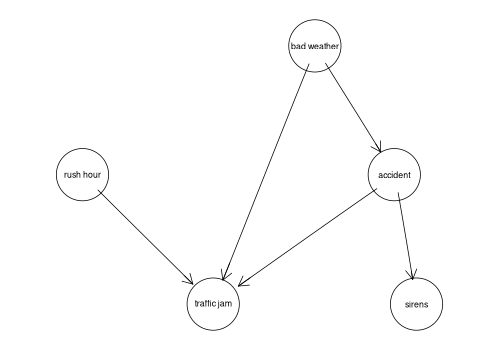
\includegraphics[width=0.8\textwidth]{images/trafficjam.png}
  \caption{An example of a simple DAG \parencite{traffic_jam}}
  \label{dag1}
\end{figure}

Each arc represents a conditional probability relationship. Nodes in the graph are assumed to be conditionally independent of all nodes which are not its parents. For example, in figure \ref{dag1}: 

\begin{equation}
  \label{eq1}
  p(sirens | data) = p(sirens | accident)
\end{equation}

These conditional probabilities are abstract in the sense that they could be treated as either discrete or continuous, and any distributional assumption of choice could be applied to them. While much of the literature surrounding Bayesian networks focuses on the discrete case, in many economic applications we are generally dealing with continuous variables. This is possible as long as we are willing to make some assumptions about the nature of the conditional probability (as truly non-parametric estimation of continuous variables implies an intractably large search space). The most common assumption here (and fortunately the most natural economic one), is that the conditional distributions follow a multivariate normal distribution of the conditioning variables. This is implies the familiar form that conditional distributions are linear functions of conditioning variables with Gaussian errors, which is exactly the assumptions of simple, small-sample OLS regression. Such models are sometimes known as "Gaussian Bayesian networks." (GBN) For example:

\begin{equation}
  \label{eq2}
  sirens|data = sirens|accident = \alpha + \beta accident + \epsilon, \space \epsilon \sim N(0, \sigma^2)
\end{equation}

Therefore,this technique is "non-parametric" in the sense that we do not make any assumptions about which underlying relationships exist between variables (indeed, this is what we hope the model will tell us). However, we do make a distributional assumption about the conditional distributions.

When fully specified, a GBN consists of a system of linear equations that defines the joint distribution of the data. Because of the properties of the normal distribution, this means that we can express a GBN as a single joint normal distribution over the data, where the DAG specifies the exact restrictions that are imposed on the variance-covariance matrix. In order to enhance clarity of exposition,in this paper all Bayesian networks are assumed to be Gaussian unless otherwise specified. The primary benefit of this simplification is the fact that uncorrelatedness implies independence, although it is by no means necessary, and many of the same results hold for arbitrary distributional assumptions.

\subsection{Estimation and Identifiabiliy}

\subsubsection{Estimation}

There are two fundamental problems to solve when estimating a DAG. The first is known as "Parameter Learning," and the other "Structure Learning." Given a DAG as in Figure \ref{dag1}, the first task is simply to estimate the parameters of the network, such as $\alpha$ and $\beta$ in Equation \ref{eq2}. This is usually done via maximum likelihood, however, other "score" functions are available such as the Bayesian Information Criterion (BIC) \parencite{chen1998speaker}.

\begin{figure}
  \centering
  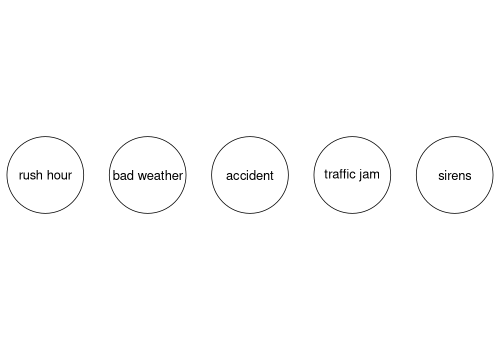
\includegraphics[width=0.8\textwidth]{images/trafficjam_unfit.png}
  \caption{A DAG before structure learning}
  \label{dag2}
\end{figure}

The second task, as demonstrated by Figure \ref{dag2} is that if we just start with some data it is not obvious which conditional probabilities to estimate in the first place. One way of achieving this is for the researcher to specify explicitly which conditional probabilities should be present in the graph, and simply fit the parameters of that graph. This however, is not what I am particularly interested in. If this is done the researcher has effectively specified a system of linear regressions to be estimated, probably based on some economic model that they already had in mind, and while this is then automatically encapsulated in a convenient, easily interpreted representation of the underlying assumptions, it seems nothing of profound economic significance is achieved in this case. 

A more more exciting approach is to algorithmically learn the structure of the graph, that is to learn a structural model, directly from observed data. One "brute force" method to solving this problem is to compute the posterior likelihood of every possible network, however, this number is super-exponential in the number of variables such that it becomes very computationally expensive, very quickly \parencite{chickering1996learning}. As a response to this, many heuristic approximation techniques have been developed. These can be grouped into two categories: constraint-based and score-based structure learning algorithms \parencite{spirtes1991algorithm} \parencite{verma1991equivalence}. 

\begin{figure}

  \centering
  \begin{subfigure}{0.3\textwidth}
    \centering
    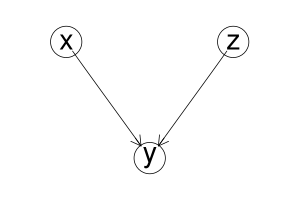
\includegraphics[width=\linewidth]{images/collider.png} 
    \small
    \begin{equation*}
      x = \epsilon_{x}
    \end{equation*}
    \begin{equation*}
      y = \alpha_y + \beta_{yx} x + \beta_{yz} z + \epsilon_{y}
    \end{equation*}
    \begin{equation*}
      z = \epsilon_{z}
    \end{equation*}
    \caption{Collider}
    \label{collider}
  \end{subfigure}
  %
  \begin{subfigure}{0.3\textwidth}
    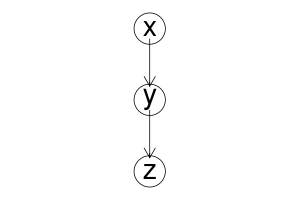
\includegraphics[width=\linewidth]{images/chain.png}
    \small
    \begin{equation*}
      x = \epsilon_{x}
    \end{equation*}
    \begin{equation*}
      y = \alpha_y + \beta_{yx} x + \epsilon_{y}
    \end{equation*}
    \begin{equation*}
      z = \alpha_z + \beta_{zy} y + \epsilon_{z}
    \end{equation*}
    \caption{Chain}
    \label{chain}
  \end{subfigure}
  %
  \begin{subfigure}{0.3\textwidth}
    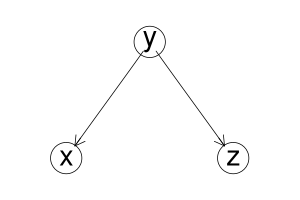
\includegraphics[width=\linewidth]{images/fork.png}
    \small
    \begin{equation*}
      x = \alpha_x + \beta_{xy} y + \epsilon_{x}
    \end{equation*}
    \begin{equation*}
      y = \epsilon_{y}
    \end{equation*}
    \begin{equation*}
      z = \alpha_z + \beta_{zy} y + \epsilon_{z}
    \end{equation*}
    \caption{Fork}
    \label{fork}
  \end{subfigure}

  \caption{The three possible V-structures of a 3 node DAG. Error terms $\epsilon$ are all i.i.d. Gaussian shocks.}
  \label{dag5}
\end{figure}

Constraint-based algorithms rely on the fact that changing the direction of an arc changes the conditional independences implied by the graph, the presence of which can be tested for in the data. To see how the DAG assumptions can be sufficient to learn a causal model in this way, consider the example in figure \ref{dag5}. Suppose we have a graph with three nodes, such that no one node is completely independent from the other two (as this would make the graph trivial, and we could in any case rule out this case with an independence test). Furthermore, the graph cannot have all three possible arcs because it would either contain a cycle, or the third arc would imply a relationship which is redundant given the other two. Then the graph must have exactly two arcs. Given this, there are exactly three possible permutations of the network, which are the three shown in figure \ref{dag5}. These are known as the the three canonical "V-structures." \parencite{pearl2014probabilistic} These structures are partially identifiable from observational data because they imply different testable hypotheses about conditional independence. While the chain and fork imply that x and z are unconditionally dependent and only independent conditional on y, the collider implies exactly the opposite; that x and z are unconditionally independent and dependent conditional on y. Given some observed data we can easily test for the presence of conditional and unconditional independence using a $\chi^2$ test. The results of these tests can be used to rule out certain network structures which would be inconsistent with the observed data. Although for every set of three variables the network is only partially identifiable, full identification can (but will not always) be achieved when more variables are observed, by comparing overlapping triplets of variables and progressively reducing the set of network structures that are consistent both with the DAG assumptions and with the observed conditional independences.

Score-based methods as the name implies assign some score to every network based on its predictive accuracy and then use gradient-decent to identify the optimum network structure. There are a number of scoring functions and hill climbing algorithms that one can use to achieve this. 

The major benefit of the constraint based method is that it directly utilises conditional independence as a primitive, which is the concept of causality that Bayesian networks seek to identify. This is in contrast to score base methods, which effectively maximise the predictive accuracy of the model, and there is seemingly no guarantee that the most predictive model is the most likely causal explanation. The major benefit of score based methods on the other hand is that they will always converge to a single fully directed graph as a solution whereas constraint based methods, because V-structures are only partially identifiable, may not be able to identify a unique solution. Instead, when the graph is only partially identifiable, the algorithm will return an undirected graph, because that arc could take on face either direction and the graph would still be consistent with both the DAG assumption and the observed conditional independences. By permuting the two possible directions of each undirected arc we arrive at a set of graphs that are said to be "observationally equivalent." This is problematic because it is difficult or impossible to fit parameters to graphs that are not fully directed (see limitations section).  

Fortunately, these two methods can be combined into so called "hybrid" structure learning methods which use the strengths of both methods to counter the weaknesses of the other. In this method a score function of choice is maximised over the set of network structures that is allowable given some constraint based algorithm. This has the benefit of using conditional independence to identify causality, while also always converging to a unique, fully directed graph. In the application in this paper I have used a hybrid structure learning algorithm.

I believe that structure learning is the greatest contribution of the Bayesian network framework. Many of the topics in this paper should seem quite familiar to any econometrician because they are fundamentally the same as some basic econometric concepts, although perhaps expressed through different language. However, the novel benefit of using this method is that we are effectively able to estimate a structural model directly from the data, without first having to specify which relationships we believe should be present. This is a very powerful concept because it removes researcher bias by allowing the data to speak for itself.

\subsubsection{Identifiabiliy}

While the previous section outlined algorithms that can learn the structure of a graph it will be important to characterise the conditions under which this process can be expected to converge to a correct model of the underlying DGP. In other words, in order to believe that the DAG learned from some observed data is the correct model, what do we have to assume about the underlying DGP? Pearl (\citeyear{pearl2009causality}) defines a sufficient assumption as the "back-door criterion." A set of observed variables $z$ is said to satisfy the back-door criterion relative to $x$ and $y$ if:

\begin{enumerate}
  \item no node in $z$ is a decendent of $x$
  \item $z$ blocks every path between $x$ and $y$ that contains an arrow into $x$
\end{enumerate}

Here a path is any combination of arcs connecting one node to another (regardless of direction), and a path between $x$ and $y$ is blocked if $x$ and $y$ are independent in the DAG given $z$. Intuitively, this is the concept in economics commonly described as unconfoundedness. Although more general, it implies in particular that even if there are variables that are relevant to the true DGP that are unobserved, the DAG can still consistently estimate the causal effect of $x$ on $y$ as long as $x$ and $y$ have no common, unobserved causes (confounders). In particular, this identifying assumption allows for the causal effect of $x$ on $y$ to be observed, even if there is some unobserved variable $u$ that intermediates the causal path. This is profound in many economic applications where models assume that some unobservable function intermediates the relationships between observed variables. For example, a (unobservable) utility function intermediates the path between the observable determinants of demand such as price and preference ordering, and the quantity purchased. In this context, the front-door criterion implies that even if the true DGP contains a utility function which is unobservable to the model it is still possible correctly identify the causal effect of the demand determinants on the quantity purchased as long as all relevant determinants of the utility function are observed. The back-door criterion implies that complex functions that intermediate the relationship between observables are \textit{emergent} in the model without being explicitly assumed.

DAGs can also consistently identify a causal effect if it satisfies the "front-door criterion." A set of variables $z$ is said to satisfy the front-door criterion relative to variables $x$ and $y$ if it satisfies the following three assumptions \parencite{pearl2009causality}:

\begin{enumerate}
  \item $z$ blocks all directed paths from $x$ to $y$
  \item there are no unblocked back-door paths from $x$ to $z$
  \item all back-door paths from $z$ to $y$ are blocked by $x$
\end{enumerate}

\begin{figure}
  \centering
  \begin{subfigure}{0.45\textwidth}
    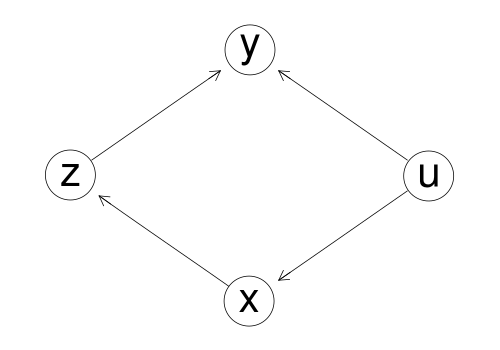
\includegraphics[width=\linewidth]{images/frontdoor.png} 
    \caption{Front-door criterion}
    \label{dag8_fd}
  \end{subfigure}
  %
  \begin{subfigure}{0.45\textwidth}
    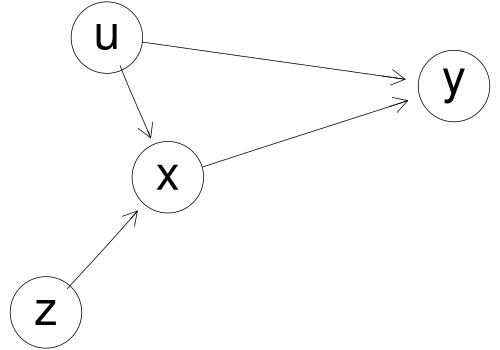
\includegraphics[width=\linewidth]{images/iv.png}
    \caption{Instrumental variables}
    \label{dag8_iv}
  \end{subfigure}
\end{figure}

The front-door criterion is demonstrated by figure \ref{dag8_fd}. Intuitively, what this allow s for is a sort of reverse instrumental variables identification where the instrument $z$ intermediates the causal path from $x$ to $y$ instead of being a parent/determinant of $x$. The assumptions here are similar in scope to those made in instrumental variables. The first assumption is akin to the exclusion restriction, the second exogeneity, and the third relevance.

Both the back-door and front-door criterion make strong assumptions about unobserved variables, which raises questions about their applicability. However, this problem is hardly specific to Bayesian networks. Empirical economists are well acquainted with the difficulty of making arguments of unconfoundedness that are also required by many traditional econometric techniques, such as the exogeneity assumption required for instrumental variables. Because DAGs are an easily scalable machine learning technique they can add a sort of "brute force" tool to the empirical economics toolbox. This technique allows for causal inference by appeal to high-dimensional data sets rather than the clever arguments and insights usually required by econometric models over a small number of observed variables.

\subsection{Causality and Inference}

Now that the mathematical underpinnings of DAGs have been introduced, it will be necessary to discuss the concept of causality that they employ, because it is somewhat different from what we are used to in economics. Most modern empirical work in economics utilises the "Potental Outcome" causal framework \parencite{holland1986statistics}. In this framework a causal effect or treatment effect is defined as the difference between an outcome for an observational unit in the presence of a treatment $Y_i(1)$, and in the absence of the treatment $Y_i(0)$. This thinking is inspired by the medical and other physical sciences, where for example, the treatment effect of a medication on a patient's blood pressure is defined as the difference between the patient's blood pressure after taking the medication and \textit{what it would have been} if they had not taken the medication. Since in reality we can only ever observe one of these contingencies many statistical techniques have been developed that are able to consistently estimate this amount. Therefore, the potential outcomes framework can be said to make statements about counterfactuals, that is, the difference between outcomes in different states of the world.

The concept of causality that is relevant to Bayesian networks is that of conditional independence. While this may seem unusual, this is actually akin to what is often assumed in macroeconomic theory, where every model has "exogenous shocks" that are the fundamental cause of the model dynamics. If we represent such macroeconomic models as DAGs these exogenous shocks would be the root nodes of the graph, because the root nodes of a Bayesian network are assumed to be distributed independently of all other variables in the graph. In this framework the primary meaning of causality is exogeneity (that is in the literal sense, not being determined by what is observed), rather than treatment effects as in the potential outcomes framework. Since both of these concepts of causality (treatment effects and exogeneity) are commonly used in the field of economics one would like to believe that they are internally consistent, and indeed as I will argue in the remainder of this section, they are not incompatible. Indeed, Bayesian networks are entirely consistent with potential outcomes and can be used to elicit counterfactuals / (average) treatment effects.

\begin{figure}
  \centering
  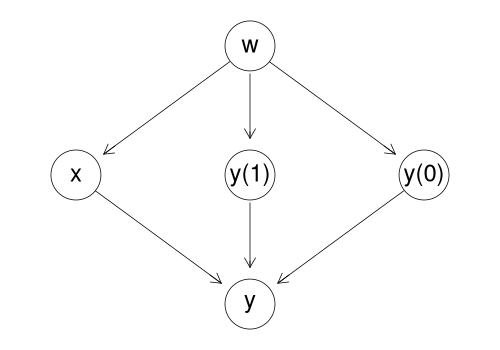
\includegraphics[width=0.8\textwidth]{images/potential_outcomes_dag.png}
  \caption{Potential Outcomes as a DAG}
  \label{dag6}
\end{figure}

Barr (\citeyear{barr2018causal}) gives an example of how the potential outcomes framework can be represented by a DAG, which is illustrated by figure \ref{dag6}. In this model, $w$ is a set of confounders, $x$ is the binary treatment of interest, $y(1)$ and $y(0)$ are the potential outcomes with and without the treatment respectively, and $y$ is $y(x)$. The fundamental assumption necessary for the consistent estimation of the average treatment effect here is that that given the confounders $w$ the treatment $x$ is independent of the potential outcomes. This is the assumption of unconfoundedness between the treatment and the treatment effects:
 
\begin{equation}
  x \perp \!\!\! \perp  (y(1), y(0)) | w
\end{equation}

In the graph, this assumption is illustrated by the fact that the only paths from $x$ to the potential outcomes are either through $y$, which is a collider which implies independence, or through $w$ which we have controlled for. This is an example of what Pearl (\citeyear{pearl2018book}) describes as the "back-door criterion" which he identifies as a necessary conditions for DAGs to have a causal interpretation. This illustrates the deep conceptual similarities between these frameworks.

Furthermore, Bayesian networks can be used to estimate counterfactual outcomes, using what Pearl (\citeyear{pearl2014probabilistic}) describes as "do-calculus." This uses the notation $P(y|do(x=\bar{x}))$. The difference between this and $P(y|x=\bar{x})$ is that $do(x=\bar{x})$ reflects an exogenous change in $x$ to $\bar{x}$, whereas $P(y|x=\bar{x})$ suggests that the model is in a state that would predict that the variable $x$ takes on the value $\bar{x}$. Under some conditions, computing $P(y|do(x=\bar{x}))$ can achieved by breaking the links of $x$ with its parents and setting it to $\bar{x}$, and then observing $y$ in the model. This is demonstrated by Figure \ref{dag3}. For example, consider Figure \ref{dag3}. Suppose for simplicity that all of the variables are binary (1 in the presence of the event, 0 otherwise). On the LHS of the diagram we have the model for observed values of all of the variables. On the RHS we intervene on "accident." Notice that doing so breaks the link between "bad weather" and "accident." We can now estimate the causal treatment effect of an accident on the probability of a traffic jam given some values of "bad weather" and "rush hour" (in other words, all else equal) according to equation \ref{eq3}. This equation is very familiar, and is effectively the same as the calculation of an average treatment effect in the potential outcomes framework.

\begin{equation}
  \label{eq3}
  p(tj | bw = \bar{bw}, rh = \bar{rh}, do(a=1)) - p(tj | bw = \bar{bw}, rh = \bar{rh}, do(a=0))
\end{equation}

\begin{figure}

  \centering
  \begin{subfigure}{0.45\textwidth}
    \centering
    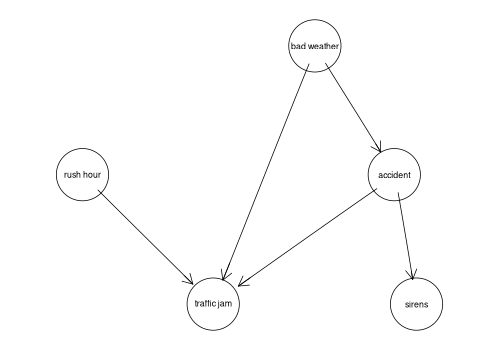
\includegraphics[width=\linewidth]{images/trafficjam.png} 
    \caption{No intervention}
  \end{subfigure}
  %
  \begin{subfigure}{0.05\textwidth}
    \centering
    $\rightarrow$
  \end{subfigure}
  %
  \begin{subfigure}{0.45\textwidth}
    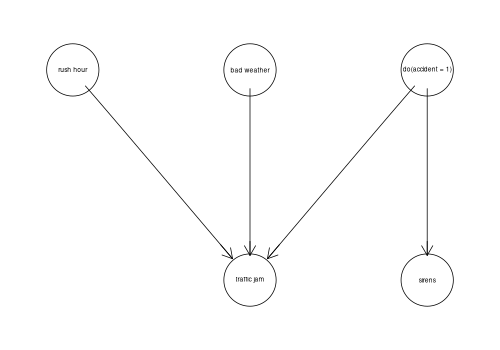
\includegraphics[width=\linewidth]{images/trafficjam_intervention.png}
    \caption{Intervention}
  \end{subfigure}

  \caption{An example of intervention}
  \label{dag3}
\end{figure}

In addition, there are other kinds of possible prediction exercises that we may be interested in with some economic interpretation. Since the model defines every endogenous variable as a (linear) function of the exogenous shocks it can be interpreted as a structural model of the data. Therefore, we might compute impulse response functions (IRFs) for each endogenous variable in the model to one or more shocks.

\subsection{Limitations}

Before continuing on to my application I would like to point out some of the limitations both of this methodology, and of my own knowledge in order to give some idea of the pitfalls that might be encountered during the course of this research. 

\subsubsection{Simultaneity}

The concept of a DAG, while a powerful tool, is not a perfect model for all data. The strongest assumption is that it is directed. In many economic applications, while we may believe that some variables are truly exogenous such that they must be causes of movement in endogenous variables and not the other way around, we usually also assume that some or all of the endogenous variables are determined in general equilibrium, that is to say there is not necessarily a directionality to every relationship between endogenous variables. The problem of simultaneity is important, but there are ways which we can work with it in the Bayesian network framework. I will propose two solutions to this problem: the first is that many relationships that we commonly think of as simultaneous have a mathematically equivalent fully directed model, and the second is that it is possible to relax the assumption that the graph is fully directed.

\begin{figure}

  \centering
  \begin{subfigure}{0.45\textwidth}
    \centering
    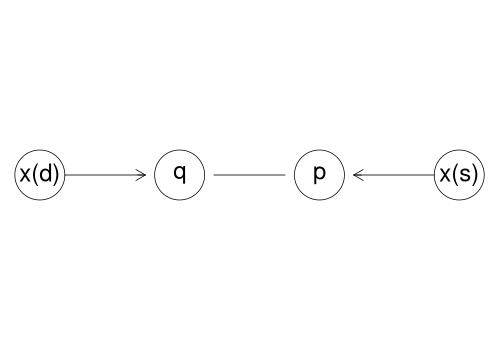
\includegraphics[width=\linewidth]{images/simultaneous.png} 
    \caption{Explcit simultaneity}
    \label{dag7_a}
  \end{subfigure}
  %
  \begin{subfigure}{0.05\textwidth}
    \centering
    $\iff$
  \end{subfigure}
  %
  \begin{subfigure}{0.45\textwidth}
    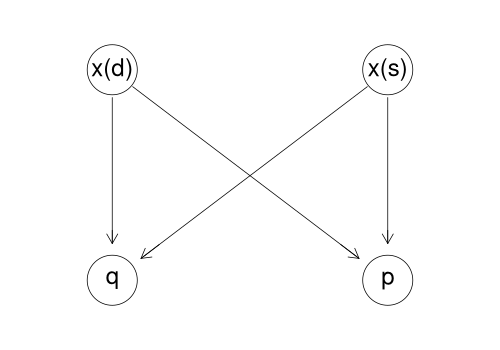
\includegraphics[width=\linewidth]{images/directed.png}
    \caption{Directed simultaneity}
    \label{dag7_b}
  \end{subfigure}

  \caption{An example of directing simultaneity}
  \label{dag7}
\end{figure}

In order to see why explicitly modelling simultaneity may not be necessary, consider figure \ref{dag7}, which is inspired by Imbens (\citeyear{imbens2019potential}). Figure \ref{dag7_a} shows a simple model of supply and demand where quantity $q$ and price $p$ are determined simultaneously in the presence of demand shock $x(d)$ and supply shock $x(s)$. The relationship between quantity and price is simultaneous because changes in each one affect the other. However, the relationships implied by figure \ref{dag7_a} can just as well be represented by the fully directed graph in figure \ref{dag7_b}. To see this consider the following equations which are implied by figure \ref{dag7_a}:

\begin{equation}
  p = \alpha_p + \beta_{ps} x(s) + \beta_{pq} q + \epsilon_{p}
\end{equation}
\begin{equation}
  q = \alpha_q + \beta_{qd} x(d) + \beta_{qp} p + \epsilon_{q}
\end{equation}

By substituting $p$ into the equation for $q$ and vice versa it can be shown that this system of equations is equivalent to:

\begin{equation}
  \label{price_eq}
  p = \frac{1}{1-\beta_{pq}\beta_{qp}}[(\alpha_p + \beta_{pq} \alpha_q) + \beta_{ps} x(s) + \beta_{pq} \beta_{qd} x(d) + (\epsilon_p + \beta_{pq} \epsilon_q)]
\end{equation}
\begin{equation}
  \label{quantity_eq}
  q = \frac{1}{1-\beta_{qp}\beta_{pq}}[(\alpha_q + \beta_{qp} \alpha_p) + \beta_{qd} x(d) + \beta_{qp} \beta_{ps} x(s) + (\epsilon_q + \beta_{qp} \epsilon_p)]
\end{equation}

Which is (a version of) what is represented by figure \ref{dag7_b}. At this point I will note the relevance of the Lucas (\citeyear{lucas1976econometric}) critique. The model in \ref{dag7_b} is a reduced form estimation of the model in \ref{dag7_a}, and as such, it will be impossible to identify the policy parameters $\beta_{pq}$ and $\beta_{qp}$. In general, DAGs are a statistical technique that rely only on observed data, and therefore, they will not be immune to the Lucas critique. However, we \textit{can} identify the impact of exogenous shocks to the model. In the context of this example, this means that while the DAG cannot consistently estimate the supply and demand elasticities, it can consistently estimate the effect of a demand shock $x(d)$ or supply shock $x(s)$ on the equilibrium of the model. In the context of macroeconomic models we are often interested in computing IRFs which is the equilibrium effect of an exogenous shock to the model. This argument illustrates why even though we believe that many of the variables in these macroeconomic models are simultaneously determined, we can still estimate IRFs using DAGs. More generally, although DAGs might not be able to identify all structural parameters that economists might be interested in, they are nonetheless able to identify causal effects and in many applications this is likely sufficient. 

However, it is also possible to explicitly model simultaneity in the context of graphical models. As discussed earlier, constraint based structure learning algorithms do not force a direction onto every arc, so it is entirely possible for sturcure learning to result in a Partially Directed Acyclical Graph (PDAG). Such models are known as hybrid networks or chain graphs, originally proposed by Wermuth and Lauritzen (\citeyear{wermuth1990substantive}). Recall that the DAG assumption can be characterised as a set of constraints on the covariance matrix of the joint normal distribution. In a hybrid network then there are no constraints on the partition of the covaraince matrix for the variables in the model that are assumed to be simultaneous. Note however, that while this approach may be more comfortable from the economic point of view it will still not immunise the model to the Lucas critique. Unfortunately, I was unable to find any convincing implementations which allow for hybrid networks. Therefore, all of the graphs that I use in my application are fully directed and used with appeal to the previous argument.

Through my experimentation with these methods I have also had a lot of mixed results. I have tried to perform this type of analysis for a few models, and it does not seem to work well for all of them. In the next section I will discuss the results for a baseline RBC model for which the results have been rather promising. On the other hand, I have attempted to model the medium-scale New Keynesian model from \parencite{smets2007shocks}, without much success. In this model there are a large number of variables, many of which seem to actually measure the same thing, so it is hardly surprising that the algorithm becomes confused. Therefore, at this time I will not completely write this one off. On the contrary, I bring this up to point out that while this is potentially a very useful modelling technique it is not a "magic bullet." Some assumptions on input data will be required. It is likely that some substantial part of my thesis will be dedicated to understanding in what situations Bayesian networks work well, as well as what assumptions might be needed to guarantee that a faithful DAG can/will be found.

Upon first being exposed to these ideas many are critical whether it is even conceptually possible to make such causal inferences directly from data. The section on structure learning gives some very brief overview of how we try to go about practically solving this problem. As far as the conceptual problem is concerned I do not yet understand it well enough myself to make a compelling argument. It is clear that going forward with this research will require me to do much deeper reading about the justification of direct structural learning. However, being the pragmatist that I am, it is for this reason that I have chosen to perform some direct applications in order to demonstrate simply whether or not such a strategy is likely to bear fruit, regardless of the strength of its theoretical underpinnings. The results so far have not been perfect, but I believe it has been successful enough to warrant further investigation into this topic.

\section{Application}

\subsection{Data}

In order to demonstrate the capability of the Bayesian network method empirically I have chosen to use simulated data from macroeconomic models. This is not completely arbitrary; I envisage using simulated along with real macroeconomic data in my actual thesis. There are a few key reasons why I have chosen to work with this data. Firstly, since the model that simulates the data is known it is possible to evaluate whether the structure learning has succeeded in identifying the underlying relationships in the data. In other words, since the true DGP is known it is possible to infer whether the estimated DAG faithfully represents the underlying DGP. Secondly, in the context of a log-linearized macroeconomic model the parametric assumptions (that conditional distributions are linear with Gaussian errors) are in fact correct. Finally, and more personally, given the choice of an application in microeconomics or macroeconomics I prefer one in macroeconomics because that is what I find more interesting.

\subsection{Methodology}

In order to collect this data I have found a repository of Dynare code for simulating many well-known macroeconomic DSGE models \parencite{pfeifer2020}. I then modified this code slightly such that the output would be a data file containing simulated values of i.i.d. shocks and endogenous variables. I then load this data into R, and using the "bnlearn" package \parencite{scutari2020}, I fit a Bayesian network, using a hybrid algorithm to learn the structure because there are theoretical advantages that I outlined in the section on structure learning and it seemed to perform best in my short experimentation. Finally, I estimate the parameters of the model using maximum likelihood. Once the model is fit I perform a few experiments to evaluate the model performance.

\subsection{Results}

The data that I have used in this comes from a relatively detailed RBC model with a good number of variables to study. Table \ref{tab1} gives a summary of the variables in the data. In this model "z" and "g" are exogenous and each follow and independent i.i.d. Gaussian process. Capital is also exogenous in period t because it is chosen (endogenously) in period t-1. In general, we could include lags of some or all variables in order to take dynamics into account, but I will leave that for future investigation. For the sake of space, I will forego any further discussion of the relationships between endogenous variables, stating simply that these are of the standard RBC nature.

\begin{table}
  \centering
  \begin{tabular}{|l|l|l|}
    \hline
    Symbol & Name & Exogenous? \\
    \hline
    g & government spending & yes \\
    z & technology process & yes \\
    k & capital & yes \\
    w & wage rate & no \\
    r & return to capital & no \\
    y & output & no \\
    c & consumption & no \\
    l & hours worked & no \\
    i & investment & no \\ \cline{2-2}
    \hline
  \end{tabular}
  \caption{Description of Variables}
  \label{tab1}
\end{table}

\begin{figure}
  \centering
  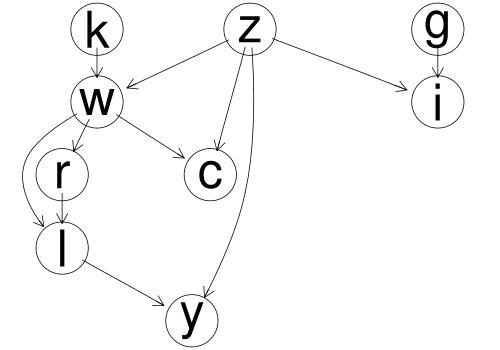
\includegraphics[width=\textwidth, height=0.25\textheight, keepaspectratio]{images/rbc_dag.png}
  \caption{Structure of DAG fit to RBC data}
  \label{rbcdag}
\end{figure}

\begin{figure}
  \centering
  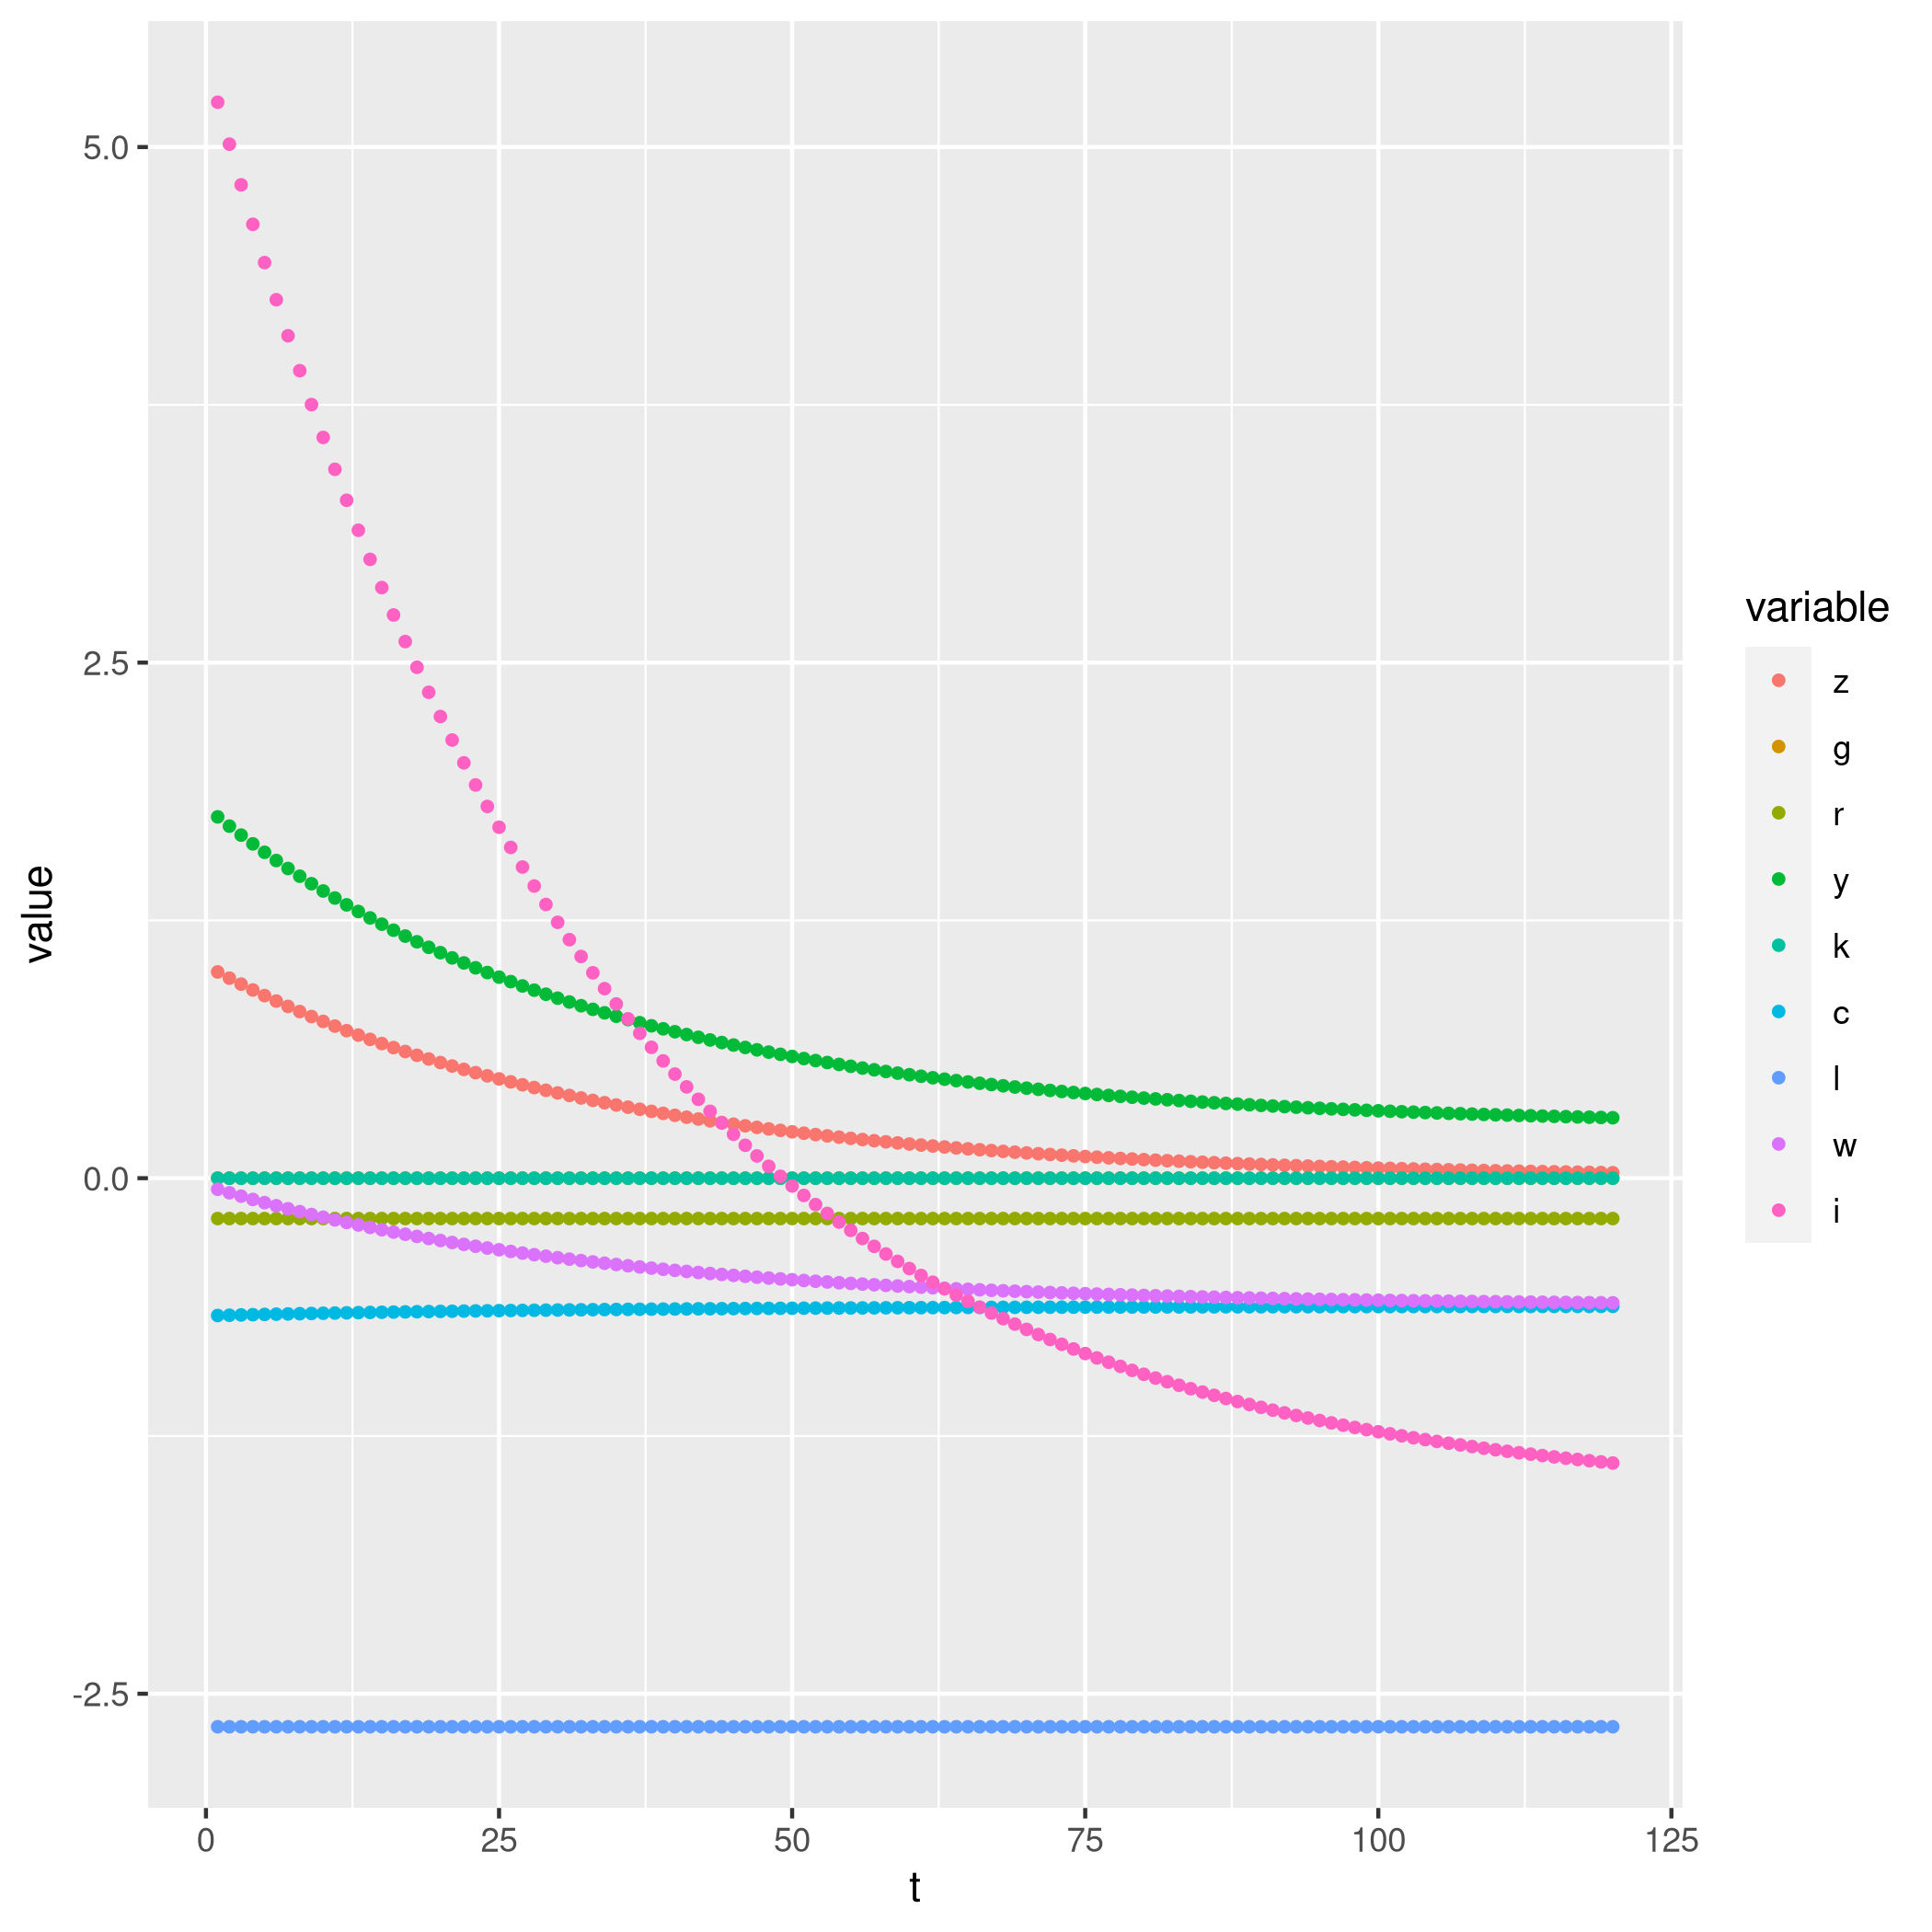
\includegraphics[width=\textwidth, height=0.4\textheight, keepaspectratio]{images/rbc_irf.png}
  \caption{IRFs to technology shock predicted by model}
  \label{rbcirf}
\end{figure}

Figure \ref{rbcdag} shows the structure of the DAG that was fit to the RBC data, with a sample size of 200. Here we note that structure learning successfully identified the three exogenous variables in the model as root nodes. Since the graph is fully directed we are able to fit parameters to the model in order to perform predictions. For example, we can perform pure prediction on output. In the spirit of best practice for machine learning we split the data into training and test data sets, and use only the training data to fit the parameters of the model. When doing this we find that the accuracy of predicting any endogenous variable in the test data is extremely high ($R^2 \approx 1$), although it should be noted that the variables are perfectly co-linear, so this prediction exercise is not exactly challenging. 

A more interesting exercise is to compute IRFs for the endogenous variables. Figure \ref{rbcirf} shows the result of computing IRFs for endogenous variables to a positive $AR(1)$ technology shock of one standard deviation. This is calculated by setting the value of "z" to decay by $\alpha_z$ every period from an initial value of 1 standard deviation, setting the other shocks to 0, and then calculating the predicted values for all of the endogenous variables\footnote{Note that "l" is excluded because the model thinks it is exogenous.}. Therefore, each period we are calculating the estimated treatment effect on every endogenous variable of an exogenous technology shock, all else equal. While not perfect, qualitatively, the results are much what we would expect to see from an RBC model. For example, we can observe the standard result that investment reacts much more strongly than other variables to a technology shock.

\section{(Sketch) Research Plan}
There are a few ways that I can see taking this research, both theoretically and empirically. \citeauthor{imbens2019potential} (\citeyear{imbens2019potential}) gives a detailed account of many of the limitations to the application of DAGs in economics, and therefore, I see a great opportunity to make a significant contribution by addressing some or all of these issues in my thesis. Some of the main issues he raises, which I have already outlined my plan to address in this paper are the lack of empirical examples, inability to perform inference, and inability to handle simultaneity.

In addition to this, I would like to look at trying to identify under which conditions structure and parameter learning algorithms are likely to succeed in finding an accurate model for the data. I will investigate the various structure learning algorithms in each category and compare them theoretically and empirically. Ideally I would be able to specify precise conditions under which there theoretical guarantees of convergence can be given. This need not be done from scratch because many of these theoretical properties are already understood in the statistics literature. The key would therefore be to translate these properties into relevant constraints on economic models.

In general, I will need to do a good amount of work in order to relate these new concepts to existing ones in the economics literature. For example, we can think of the Bayesian network as imposing certain restrictions on the covariance matrix of the assumed joint normal distribution of observed variables. Therefore, in order to get a better understanding of the economic content of these assumptions it would be a worthwhile exercise to describe in general how these restrictions compare to a Cholesky decomposition, especially in the case where the Bayesian network is dynamic. 

If it is impossible to guarantee structure learning algorithms will perform reliably, and they do not seem to do so empirically, I could continue by fully or partially (by blacklisting certain arcs), manually specifying the network structure. While I think this would be less interesting (because I have already argued that structure learning is probably the most exiting thing about Bayesian networks), I still think this research would be worth pursuing because there are quite a few things that can be achieved once a faithful DAG is fit to the data. Since it is a structural model we can use it to calculate IRFs and compare to the original simulations to test the accuracy of the model. We can also generate random samples from the network and compare the statistical properties of these data to those of the original data.

Finally, regardless of what form the final thesis takes I intend to take it to real data. I have decided to start with simulated data because knowing the true DGP gives the opportunity to test whether structure learning is working. However, if I can succeed in making a strong argument that these algorithms can learn effectively under some conditions, then obviously the most interesting thing will be to take it to real data and see what sort of implications the model gives us.  

\printbibliography

\end{document}
